\section{Method}
\label{sec:method}
\begin{figure}[t]
\floatconts
  {fig:overview}
  {\caption{Overview of the proposed model. The analyzed tracks $P_0$ and the waveform encoder feed the shared representation $h$, from which the modal corrections $\hat{P}$, the noise-band amplitudes $a_b$, and a clip code $\mathbf{s}$ for the transient TCN are predicted. Dashed lines mark the stop-gradient input of the TCN and the post-hoc SAE edit of $h$, during which $\mathbf{s}$ keeps its unedited value.}}
  {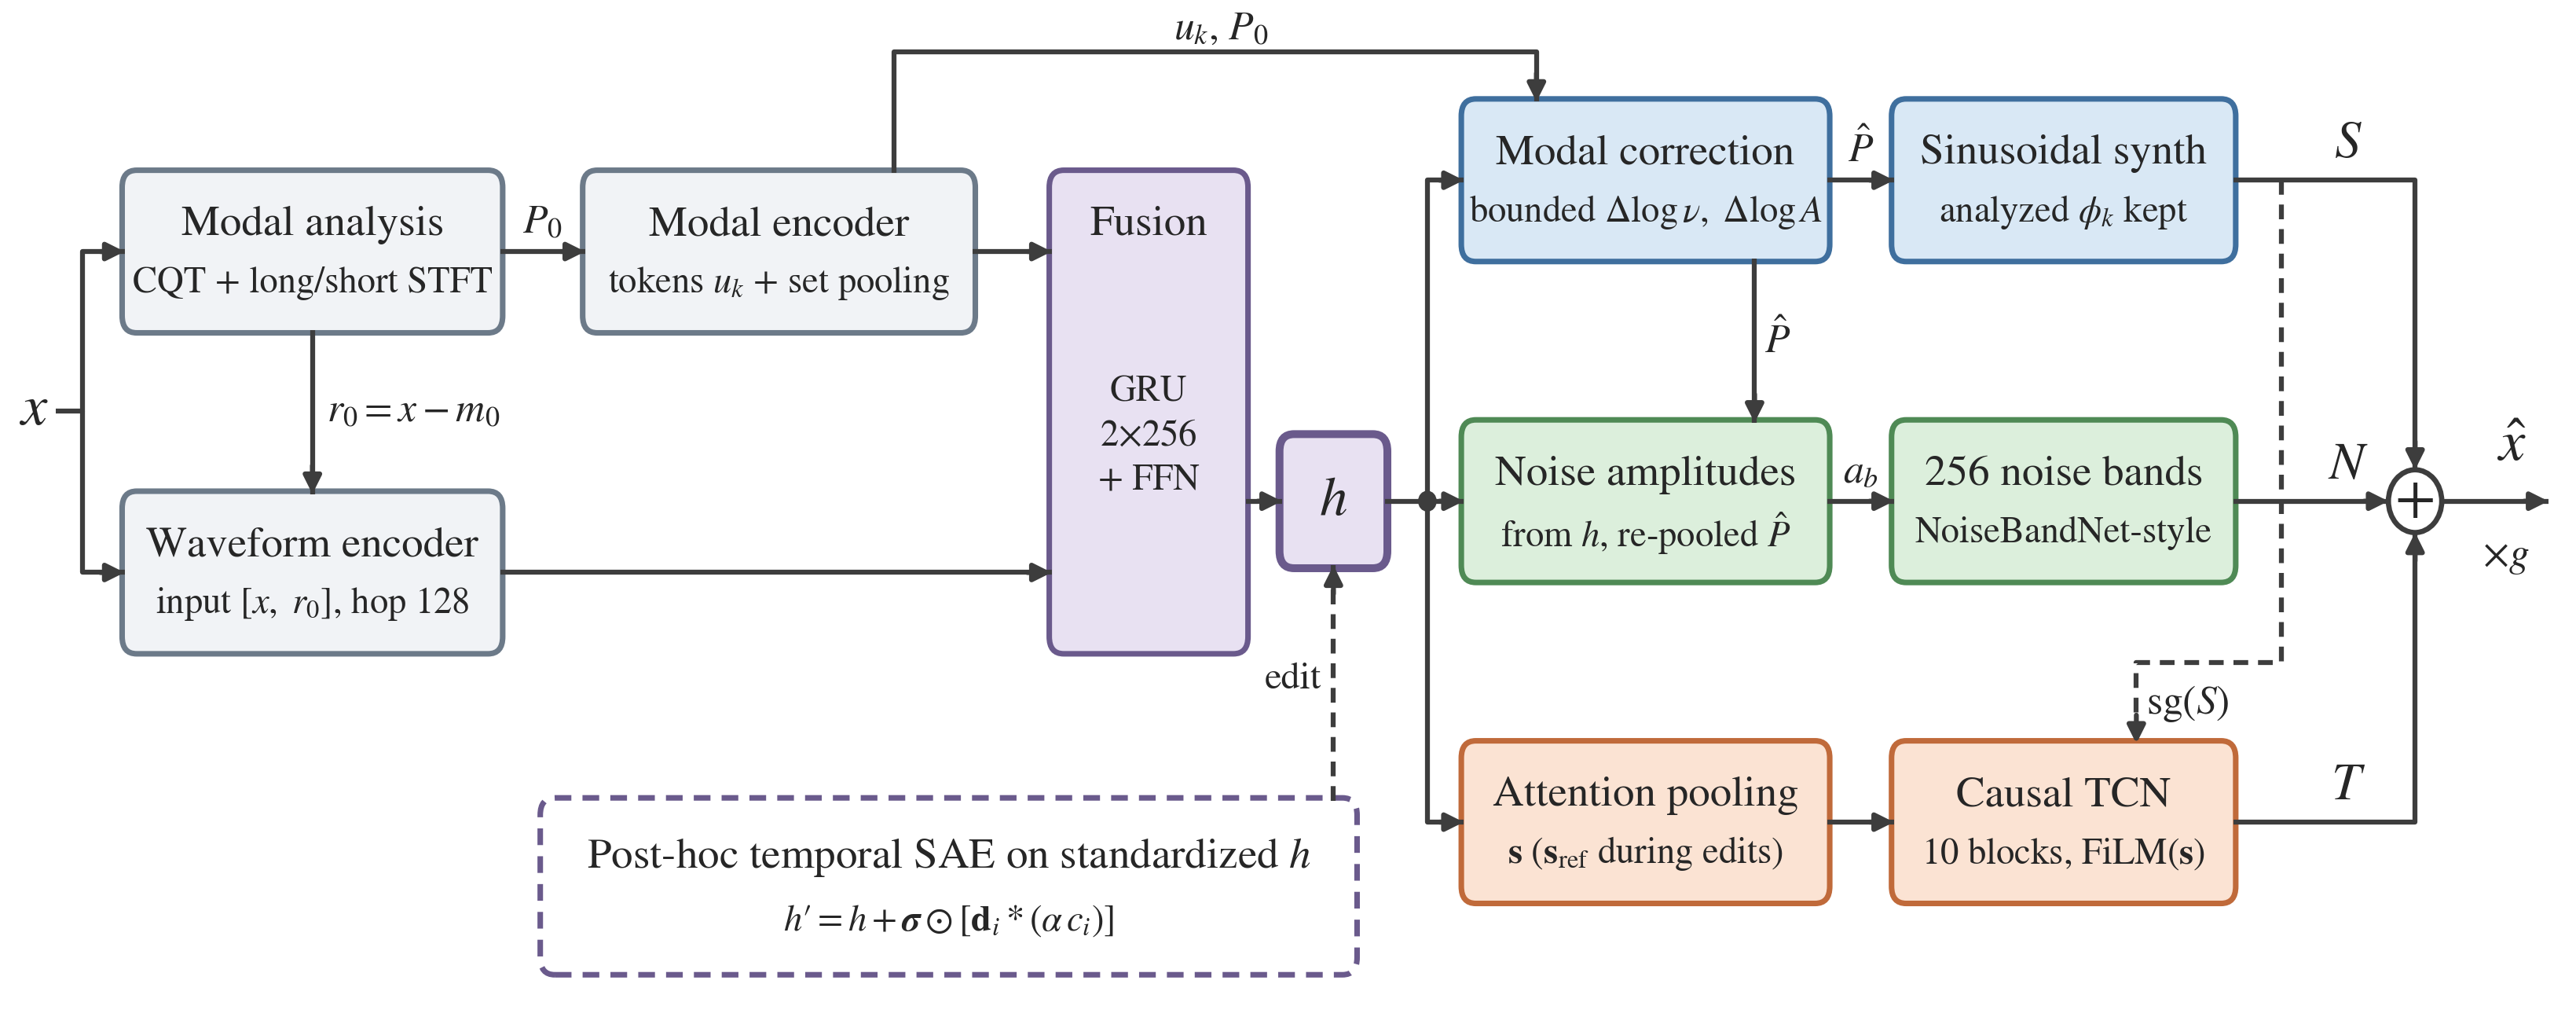
\includegraphics[width=\linewidth]{figures/figure1.png}}
\end{figure}
The proposed model reconstructs a percussive one-shot $x$ as
\begin{equation}
\hat{x} = g\,(S + N + T),
\label{eq:model}
\end{equation}
where $S$, $N$, and $T$ are the modal, noise, and transient components and $g$ is a gain shared by all three.
$S$ and $N$ are rendered by signal processing synthesizers from parameters predicted by a neural network, whereas $T$ is generated by a small TCN.
All three components are driven by one shared representation and are trained jointly through their sum, and label-free controls are later obtained from an SAE fitted to this representation.
\figureref{fig:overview} summarizes the analysis, the shared representation, the three synthesis paths, and the point at which the controls act.
The model builds on DrumBlender \citep{shier2023differentiable}: it keeps the three-component decomposition, the waveform encoder, and the modal-driven TCN, revises the modal analysis, and replaces the filtered noise with the noise bands of NoiseBandNet \citep{barahonarios2024noisebandnet}.
Signals are sampled at 48~kHz.

\subsection{Modal Analysis and Reference}
\label{sec:method-analysis}
Each sample is first analyzed into sinusoidal tracks that serve as the reference for the modal component.
DrumBlender applies the peak picking and parabolic interpolation of sinusoidal analysis \citep{serra1990spectral} to a CQT and keeps up to 64 tracks.
The CQT resolves low-frequency resonances well, but its bins widen with frequency, from about 1.8~Hz at 60~Hz to about 29~Hz at 1~kHz with 24 bins per octave.
More critically, its tracker links peaks greedily from the tail toward the onset with a tolerance of 5\% of the CQT bin index, which at 1~kHz admits any peak between about 820 and 1220~Hz and widens further at higher frequencies, so distinct peaks, such as an early peak at 1~kHz and a later one at 850~Hz, can be joined into a single gliding track.
Because DrumBlender extracts these tracks before training and renders them without correction, such merged tracks go directly into the output, where their gliding frequencies produce artifacts and the energy they wrongly assign to the modal component distorts what the noise and transient components must model.

This work therefore keeps the CQT only below 700~Hz and adds full-band STFTs whose long window resolves frequency and whose short window localizes short-lived resonances in time.
Peaks are refined by parabolic interpolation of the log magnitude \citep{smith1987parshl}, and overlapping peaks are fitted jointly.
Tracks are linked by one-to-one matching within a frequency range predicted from each track, with a cost on phase continuity.
Short or weak tracks are discarded, and at most 64 tracks are kept.
The result is a reference parameter set $P_0=\{\nu_k[j], A_k[j], \phi_k\}$ with frequency $\nu$ in cycles per sample, amplitude $A$, and initial phase $\phi_k$ for track $k$ and analysis frame $j$.

The waveform and the reference amplitudes are divided by the peak absolute value $g$ of $x$, so that the relative levels of the components are preserved when the output is rescaled in \equationref{eq:model}.
The reference modal waveform $m_0$ is rendered from $P_0$, and the reference residual is $r_0=x-m_0$; both are fixed for each sample.
The residual is given only to the waveform encoder and is not a target for the noise or transient components, because correcting the modal parameters changes which part of $x$ the modal component leaves unexplained.

\subsection{Shared Representation}
\label{sec:method-encoder}
A waveform encoder, which follows the convolutional encoder of SoundStream \citep{zeghidour2022soundstream} used in DrumBlender, receives $x$ and $r_0$ as two channels and produces one frame every 128 samples (2.67~ms at 48~kHz).
A modal encoder embeds the frequency, amplitude, and initial phase of each track and frame with a shared perceptron and processes each track along time without mixing tracks, which yields per-track tokens $u_k[j]$.
Because a track index does not refer to the same mode across samples and each token already carries its frequency and amplitude, these tokens are also summarized in each frame by attention pooling with learned queries, following the Set Transformer \citep{lee2019set}. 
The waveform features and the pooled modal context are fused and passed through a two-layer gated recurrent unit (GRU) \citep{cho2014learning} and feed-forward blocks, similar to the DDSP decoder \citep{engel2020ddsp}, to produce the shared representation $h$.
No skip connection bypasses $h$, so every learned audio feature reaches the synthesizers through $h$, which makes $h$ the single point at which the controls act.

\subsection{Synthesis Components}
\label{sec:method-synthesis}
\paragraph{Modal component.}
A correction head shared by all tracks reads each token $u_k[j]$ together with $h$ and predicts two values $q^{\mathrm{f}}_k[j]$ and $q^{\mathrm{a}}_k[j]$, which are mapped to bounded multiplicative corrections,
\begin{equation}
\hat{\nu}_k[j]=\nu_k[j]\exp\!\big(0.03\tanh q^{\mathrm{f}}_k[j]\big),\qquad
\hat{A}_k[j]=A_k[j]\exp\!\big(\log(4)\tanh q^{\mathrm{a}}_k[j]\big).
\label{eq:modal-correction}
\end{equation}
The frequency is thus corrected by at most about $\pm 52$ cents and the amplitude by a factor between $1/4$ and $4$, and the head is initialized so that the modal component initially reproduces the reference.
The corrected set is denoted by $\hat{P}=\{\hat{\nu}_k[j], \hat{A}_k[j], \phi_k\}$.
Frequency is corrected only locally because the loss surface over sinusoidal frequency is non-convex \citep{hayes2023sinusoidal}.
The correction cannot create new track.
With the parameters interpolated to audio rate and $n$ indexing samples, the modal component is
\begin{equation}
S[n]=\sum_{k}\hat{A}_k[n]\sin\!\Big(\phi_k+2\pi\sum_{m=0}^{n}\hat{\nu}_k[m]\Big),
\label{eq:modal-synth}
\end{equation}
where the initial phase $\phi_k$ stays at its analyzed value and the subsequent phase follows the corrected frequency.

\paragraph{Noise component.}
Following NoiseBandNet, the noise component is a sum of 256 fixed narrow bands with time-varying amplitudes,
\begin{equation}
N[n]=\sum_{b=1}^{256} a_b[n]\,\xi_b[n+o_b],
\label{eq:noise}
\end{equation}
where $\xi_b$ is a precomputed band-limited noise signal, read circularly from an offset $o_b$ that is random during training and fixed during evaluation, and $a_b$ is the amplitude of band $b$.
The bands are spaced linearly up to 6~kHz and logarithmically above.
The amplitudes are predicted from $h$ together with $\hat{P}$, which is summarized again with the perceptron and pooling of the modal encoder, so the noise component depends on the modal correction and its gradient also reaches that correction.

\paragraph{Transient component.}
The transient component keeps the modal-driven TCN of DrumBlender but restricts its inputs to
\begin{equation}
T=\mathrm{TCN}\big(\mathrm{sg}(S);\,\mathbf{s}\big),
\label{eq:transient}
\end{equation}
where $\mathrm{sg}$ denotes the stop-gradient operator and $\mathbf{s}$ is a single 16-dimensional vector per clip obtained by attention pooling of $h$.
The TCN consists of ten causal dilated convolution blocks with a receptive field of about 43~ms.
Each block is modulated by feature-wise linear modulation (FiLM) \citep{perez2018film} with coefficients computed once from $\mathbf{s}$, and the output layer is initialized to zero so that $T=0$ at the start of training.
Because its input is stopped, $T$ cannot pull the modal parameters through $S$, and the restriction biases $T$ toward a correction of the modal waveform without guaranteeing that it contains only the attack.

\subsection{Training Objective}
\label{sec:method-training}
The model is trained from scratch on the reconstruction of the summed output in \equationref{eq:model} with
\begin{equation}
\mathcal{L}=\mathcal{L}_{\mathrm{spec}}+\lambda_{\mathrm{env}}\,\mathcal{L}_{\mathrm{env}},\qquad \lambda_{\mathrm{env}}=0.1.
\label{eq:loss}
\end{equation}
The spectral loss is the multi-resolution STFT loss of Parallel WaveGAN \citep{yamamoto2020parallel} over four STFT sizes $M\in\{256,1024,4096,8192\}$ with Hann windows and hop $M/4$,
\begin{equation}
\mathcal{L}_{\mathrm{spec}}=\frac{1}{4}\sum_{M}\left(\frac{\lVert \hat{X}_M-X_M\rVert_F}{\lVert X_M\rVert_F}+\big\langle\,\lvert\log\hat{X}_M-\log X_M\rvert\,\big\rangle\right),
\label{eq:spec-loss}
\end{equation}
where $X_M$ and $\hat{X}_M$ are the magnitude spectrograms of the target and the reconstruction, $\langle\cdot\rangle$ denotes the mean over time-frequency bins, and both spectrograms are computed on the valid extent of each sample.
The small STFT sizes resolve the attack in time, whereas the large ones separate closely spaced modes in frequency.
The envelope loss $\mathcal{L}_{\mathrm{env}}$ is the mean absolute difference between the log RMS levels of the target and the reconstruction over 128-sample frames.
Whereas the spectral loss compares individual time-frequency bins, this term compares the overall level of each frame, so that the onset and the decay rate are constrained.

\subsection{Label-Free Controls}
\label{sec:method-control}
After reconstruction training, the model is frozen, and its shared representation $h$ is cached for each one-shot.
The channels are standardized with the mean $\boldsymbol{\mu}$ and standard deviation $\boldsymbol{\sigma}$ of the valid training frames, each weighted by the fraction of the frame occupied by audio.
A temporal SAE reconstructs this standardized representation, with a temporal convolution and frame-wise TopK activation \citep{gao2025scaling} in its encoder and unit-norm temporal atoms in its decoder.

For a reference sample, the sparse code $\mathbf{c}$ is computed once.
A knob multiplies the activation sequence $c_i$ of feature $i$ by $1+\alpha$, which gives the edited code $\mathbf{c}'$, and with decoder $D$ and atom $\mathbf{d}_i$ the edit is
\begin{equation}
\begin{aligned}
h' &= h + \boldsymbol{\sigma}\odot\big[D(\mathbf{c}')-D(\mathbf{c})\big] \\
   &= h + \boldsymbol{\sigma}\odot\big[\mathbf{d}_i * (\alpha c_i)\big],
\end{aligned}
\label{eq:edit}
\end{equation}
where $*$ is convolution over time and $\odot$ rescales the channels.
Because only the change of the decoder output is added, the reconstruction error of the SAE does not enter the edit, and every knob starts from the reconstruction of the given sample, which is returned directly at $\alpha=0$.
The TopK selection of the reference is kept fixed during a sweep, and the edit has no effect on clips in which $c_i$ is zero.

The default edit recomputes the modal corrections and noise amplitudes from $h'$ while keeping the reference clip code $\mathbf{s}_{\mathrm{ref}}$, so the transient responds only through the edited modal waveform.
For analysis, a joint-plus-strike render also recomputes $\mathbf{s}$ from $h'$ while reusing the edited modal and noise waveforms, and a strike-only render applies the same change of $\mathbf{s}$ with the neutral modal and noise waveforms.
All renders share the reference gain and noise offsets.
